\documentclass{article}

\PassOptionsToPackage{super,sort&compress}{natbib}
\usepackage[dblblindworkshop]{neurips_2025}

% Standard packages
\usepackage{adjustbox}
\usepackage[utf8]{inputenc}
\usepackage[T1]{fontenc}
\usepackage{hyperref}
\usepackage{url}
\usepackage{booktabs}
\usepackage{amsfonts}
\usepackage{amsmath}
\usepackage{amssymb}
\usepackage{nicefrac}
\usepackage{microtype}
\usepackage{xcolor}
\usepackage{graphicx}
\usepackage[font=small,labelfont=bf]{caption}
\usepackage{subcaption}
\usepackage{threeparttable}
\usepackage{algorithm}
\usepackage{algorithmicx}
\usepackage{algpseudocode}
\usepackage{array}
\usepackage{svg}
\usepackage{enumitem}

\setcitestyle{super,comma,sort&compress}

\definecolor{cb_red}{HTML}{990000}
\definecolor{cb_green}{HTML}{AAFF80}

\title{A pipeline for interpretable neural latent discovery}
\workshoptitle{Data on the Brain \& Mind}

\author{
  Jai Bhagat \\
  Sainsbury Wellcome Centre \\
  University College London \\
  \texttt{jkbhagatio@gmail.com} \\
  \And
  Anaya Pouget \\
  Sainsbury Wellcome Centre \\
  University College London \\
  \texttt{pouget.anaya@gmail.com} \\
  \And
  Sara Molas Medina \\
  University College London \\
  \texttt{saramolas18@gmail.com} \\
}

\begin{document}

\maketitle

\begin{abstract}
Mechanistic understanding of the brain requires interpretability of large-scale neuronal computations. Many latent variable model approaches excel at decoding, but produce complex, opaque latent spaces. We address this shortcoming with NLDisco, a pipeline for interpretable neural latent discovery. Motivated by successful applications of sparse dictionary learning in mechanistic interpretability, NLDisco trains sparse encoder-decoder models whose hidden layer neurons become interpretable latents. NLDisco is a flexible, user-friendly software package that supports interpretable latent discovery across recording modalities and experimental paradigms. We validate the pipeline on both synthetic and real-world data, demonstrating that it accurately recovers ground-truth features in simulated datasets while discovering meaningful representations in actual, high-yield neuronal recordings. We conclude by discussing future development and applications, emphasizing the pipeline's potential to facilitate neuroscientific discovery and a mechanistic understanding of neural computation.
\end{abstract}

\section{Introduction}

A central goal of modern neuroscience is to understand how the brain processes information to generate behavior. A promising approach is to use latent variable models (LVMs) to identify low-dimensional, interpretable representations from high-dimensional neural data. However, existing methods often require extensive hyperparameter tuning, are not easily adaptable to different data types, and lack standardized evaluation metrics. To address these challenges, we developed NLDisco, a pipeline for interpretable neural latent discovery. NLDisco is a modular, user-friendly toolkit that streamlines the process of data preprocessing, model training, and latent evaluation.

\section{Methods: The NLDisco pipeline}

\begin{figure}[h]
    \centering
    \includegraphics[width=\linewidth]{../figures/nldisco_pipeline.pdf}
    \caption{
        \textbf{The NLDisco pipeline.} \\
        \small The NLDisco pipeline has 4 stages: 1) Spatiotemporal binning and processing of neural data; 2) Training a model; 3) Evaluating the model; 4) Evaluating the model's latents for feature interpretability. Steps 1-3 can be either semi- or fully-automated.
        \vspace{-1em}
    }
    \label{figure:nldisco_pipeline}
\end{figure}

The NLDisco pipeline transforms high-dimensional neural data into a set of interpretable latents in four primary stages (\autoref{figure:nldisco_pipeline}). The first stage prepares neural data for model training, including utilities for binning, and normalizing spike times. The second stage involves training a sparse dictionary neural network (SDNN) to reconstruct the neural data from a set of sparsely active dictionary elements. The model can be configured as an autoencoder, transcoder, or crosscoder. We use a Matryoshka architecture to learn a multi-scale feature representation, and batch top-k sparsity to enforce sparsity without a tunable regularization coefficient. An optional self-attention layer can be used to integrate information across time. The third and fourth stages involve model and latent evaluation, respectively.

\begin{figure}[tbph]
    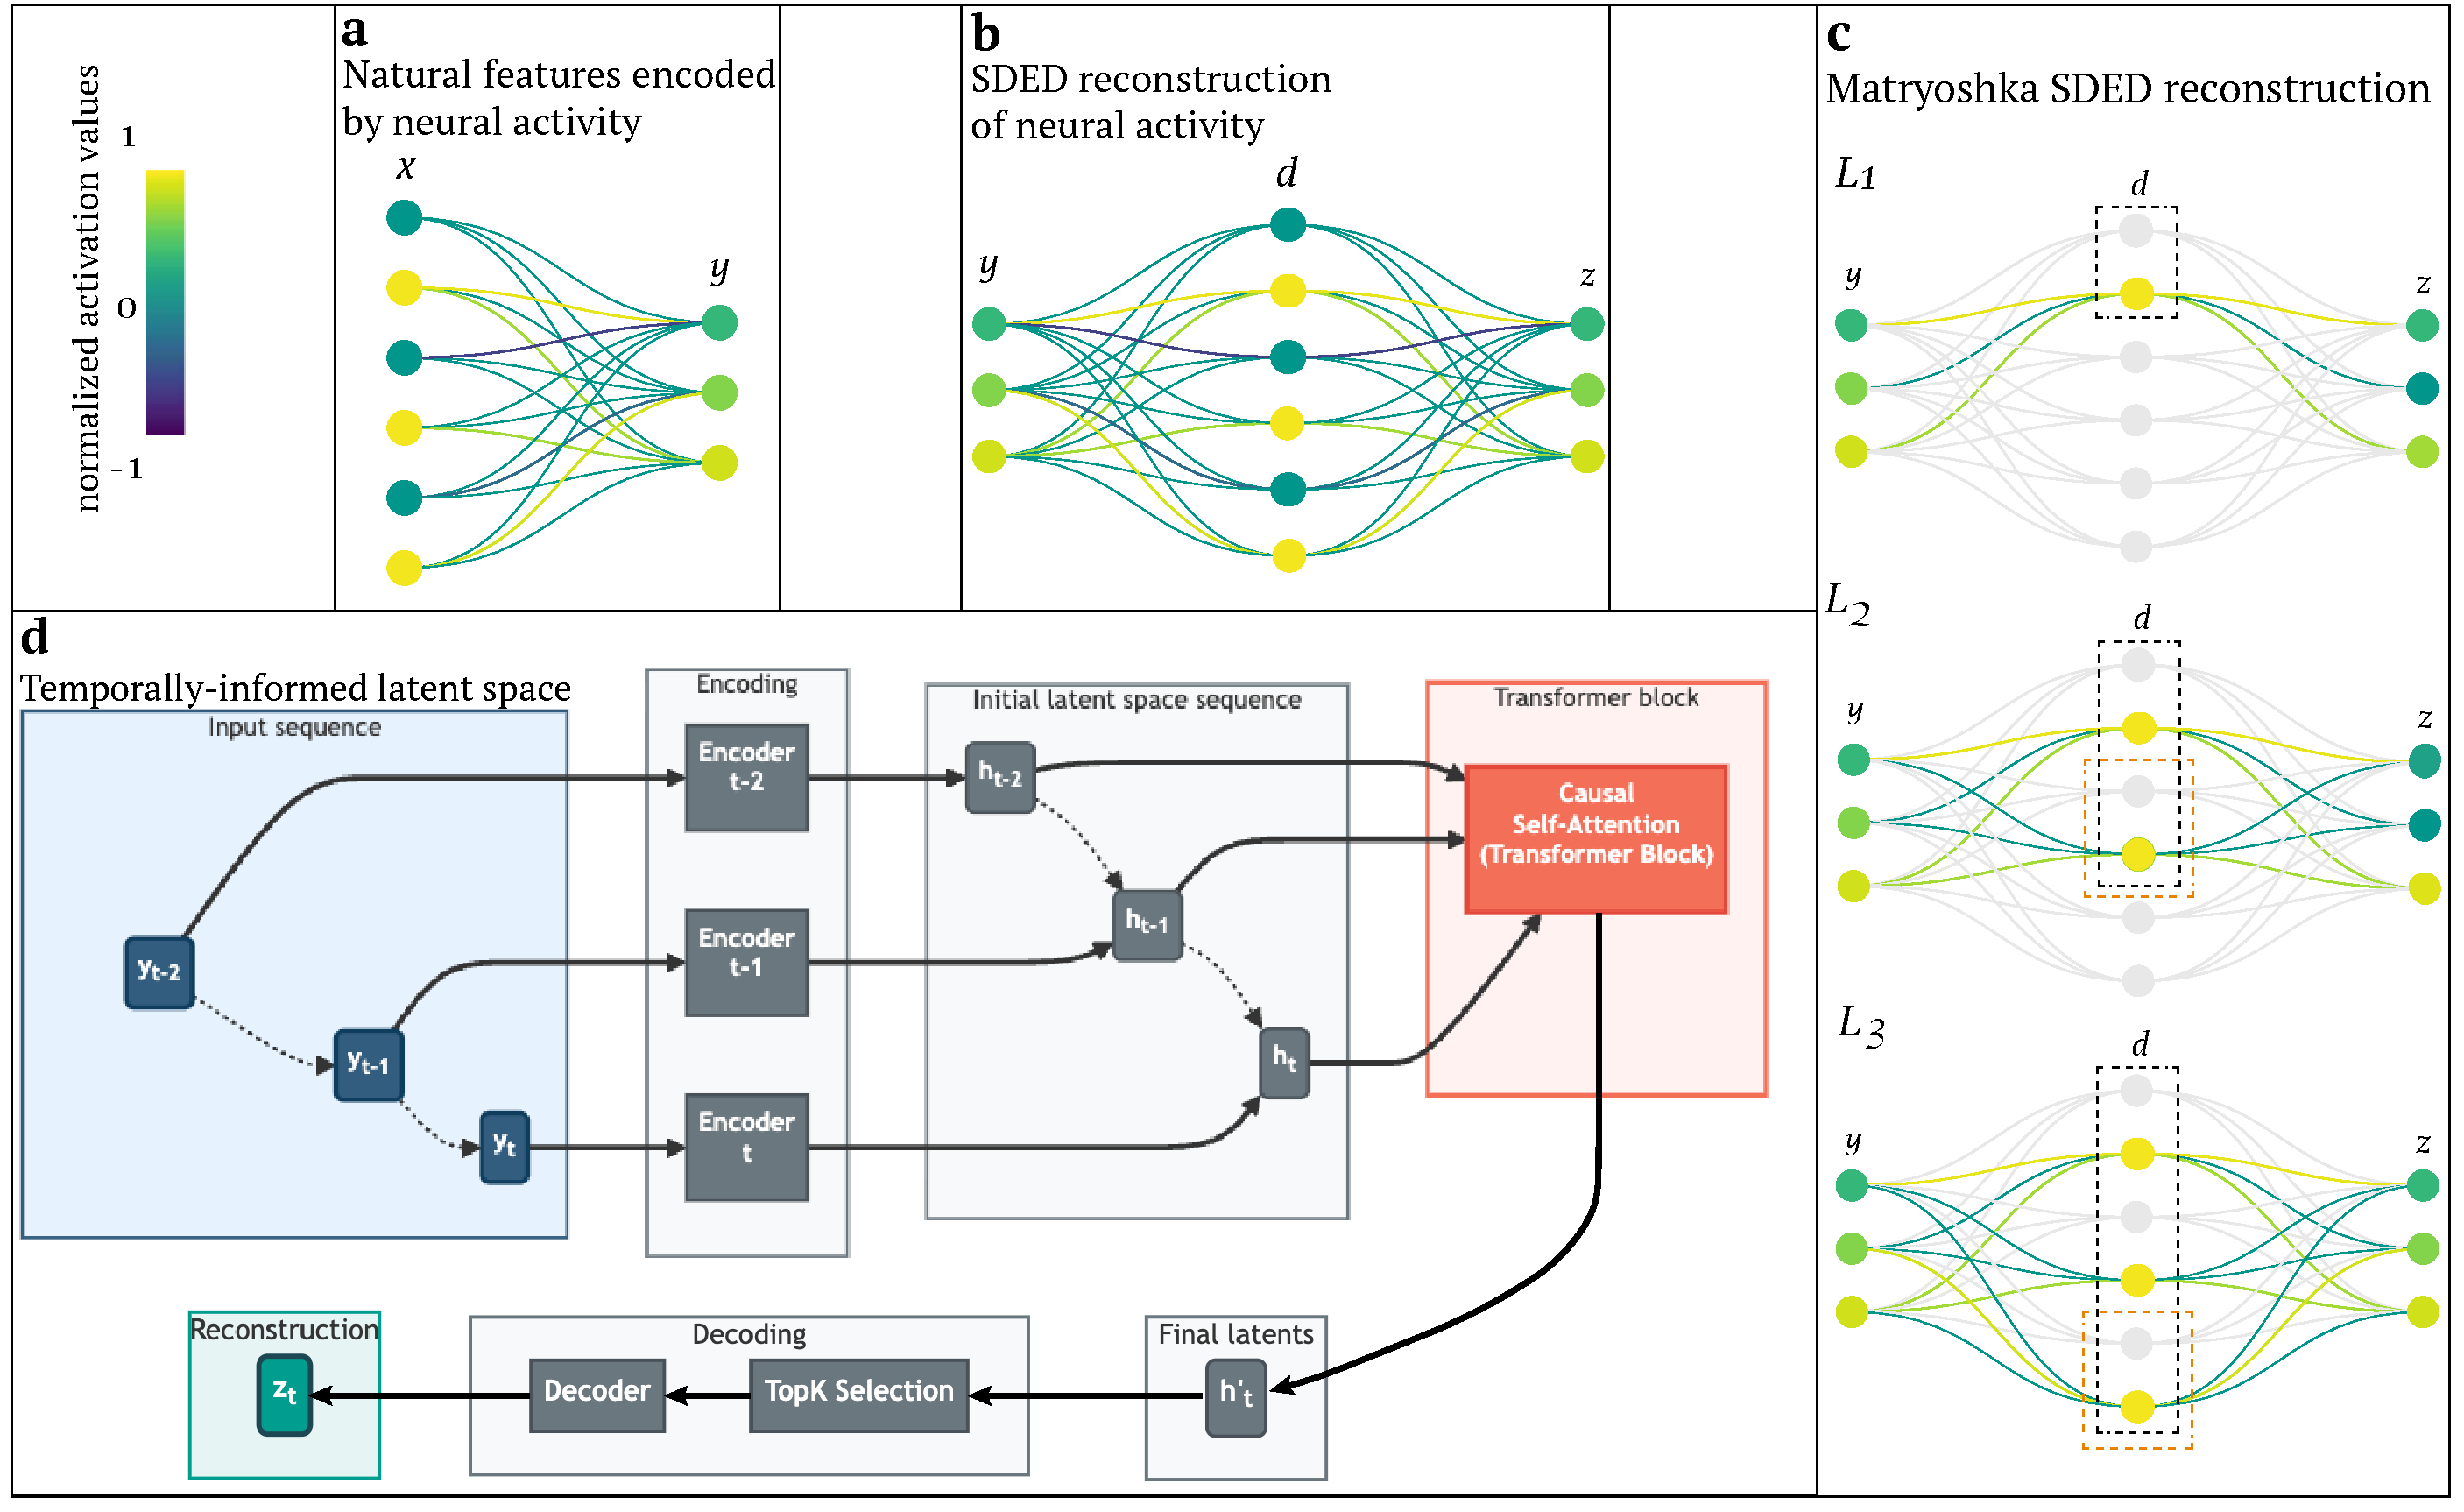
\includegraphics[width=\linewidth]{../figures/sded_arch.pdf}
    \caption{
        \textbf{Model architecture considerations} \\
        \small
        (\textbf{a}) Natural, "real-world" features $x$ are encoded by neural activity $y$. In this example, three active features are simultaneously represented by the joint activity of three neurons. (\textbf{b}) A SDED reconstructs neural activity $z$ based on $y$ via sparse dictionary elements $d$. When training is successful, $d$ corresponds to $x$: sparse dictionary elements (i.e. model neurons) represent natural features. If $z$ tries to recreate $y$ exactly ($\hat{y}$), the model is an autoencoder; in other scenarios (e.g. $z$ is separate but dependent on or related to $y$) it is a transcoder. (\textbf{c}) A Matryoshka SDED segments the latent space into multiple nested levels, each of which attempts to do a full reconstruction of the target neural activity. The black boxes indicate the latents involved in a single level, while the light-red boxes indicate the additional latents used at lower-levels. In this example, $k$=1 for top-$k$ selection of latents to recruit for reconstruction at each level (the yellow neuron within each light-red box). Latents in the highest-level ($L_1$) will often correspond to high-level features (e.g. a round object), while latents exclusive to the lowest-level ($L_3$) will often correspond to low-level features (e.g. a basketball). (\textbf{d}) Incorporation of a transformer block with sequence input allows imbuing the latents with temporal information corresponding to the evolution of the sequence, which can lead to improved reconstruction and interpretability. Each sample in the input sequence is transformed by the same encoding dictionary matrix in parallel to yield a latent space sequence. Causal self-attention is then performed on this sequence of latents via a single, small multi-head transformer block, yielding a final latent space. The latents are sparsified via top-k and transformed by the decoding dictionary matrix to yield the neural data reconstruction, as in the single, non-sequential input case.
        \vspace{-1em}
    }
    \label{figure:sded_arch}
\end{figure}

\bibliographystyle{unsrt}
\bibliography{references}

\end{document}
